\documentclass[12pt,a4paper]{article}
\usepackage[utf8]{inputenc}
\usepackage[russian]{babel}
\usepackage{amsmath}
\usepackage[obeyspaces]{url}
\usepackage{graphicx}
\graphicspath{ {./img/} }
\usepackage{listings}
\usepackage{color}
\usepackage{verbatim}
\usepackage{listings}

\definecolor{dkgreen}{rgb}{0,0.6,0}
\definecolor{gray}{rgb}{0.5,0.5,0.5}
\definecolor{mauve}{rgb}{0.58,0,0.82}

\lstset{frame=tb,
  language=Java,
  aboveskip=3mm,
  belowskip=3mm,
  showstringspaces=false,
  columns=flexible,
  basicstyle={\small\ttfamily},
  numbers=none,
  numberstyle=\tiny\color{gray},
  keywordstyle=\color{blue},
  commentstyle=\color{dkgreen},
  stringstyle=\color{mauve},
  breaklines=true,
  breakatwhitespace=true,
  tabsize=3
}


\title{Cжатие хранимых даннных методом блочной дедупликации многомерной регрессией}
\author{juhnowski@gmail.com}
\begin{document}
\maketitle
\section{ПРОБЛЕМАТИКА}

Темпы роста объема данных (файлов на ФС) $dS_{DB}$ превышают планы по закупкам вычислительнных мощностей организаций $dS_{Plan}$ из-за медленного, чем ожидалось снижения стоимости оборудования: 
  \begin{align}
    \frac{dS_{DB}}{dt} \geq \frac{dS_{Plan}}{dt} 
  \end{align}

Применение фуннкции сжатия баз данных $C(S)$ является одним из решений этой проблемы -  уменьшением хранимого размера БД $S_{DB}$:
\begin{align}
    C(S_{DB}) \leq S_{DB}
\end{align}

, настолько, что:
  \begin{align}
    \frac{dC(S_{DB})}{dt} \leq \frac{dS_{Plan}}{dt} 
  \end{align}

Для хранения баз данных, помимо экономии места, сжатие сокращает количество страниц $P_{FS}$, на которых размещаются данные, что помогает:
\begin{itemize}
    \item  сократить количество дисковых операций ввода-вывода $N_{Disk}$
 
    \begin{align}
    \frac{dN_{Disk}(C(S_{DB})}{dt} \leq \frac{dN_{Disk}(S_{DB})}{dt} 
  \end{align}

    \item повысить производительность 
 \end{itemize}

  \begin{align}
    \frac{dP_{FS}(C(S_{DB})}{dt} \leq \frac{dP_{FS}(S_{DB})}{dt} 
  \end{align}

 Для распределенных баз данных, реплицированных по географическим регионам, также существует острая необходимость в сокращении объема передачи данных $S_{Net}$, используемого для синхронизации реплик:
  \begin{align}
    \frac{dS_{Net}(C(S_{DB})}{dt} \leq \frac{dS_{Net}(S_{DB})}{dt} 
  \end{align}

Наиболее широко используемый подход к сокращению объема данных в операционных СУБД — это сжатие на уровне блоков \cite{Cormack85}, \cite{Iyer94} .

Сейчас СХД, например Huawei OceanStor \url{https://www.huawei-networks.ru/catalog/oceanstor-dorado-v6} предлагает:

\begin{itemize}
    \item В тестах с виртуализированными средами (VMware vSphere) коэффициент дедупликации достигает 5:1 — 10:1 , сжатие — 2:1 — 3:1 .

    \item В тестах с базами данных (например, Oracle, SQL Server) коэффициент дедупликации ниже (около 2:1 – 3:1 ), но сжатие сохраняется на уровне 2:1 – 3:1 .

    \item Для неструктурированных данных (например, видеофайлов) коэффициент дедупликации ниже 2:1.
\end{itemize}

Поэтому, существующими аппаратнными или программнно-аппаратнными комплексами проблема не решается.

Конечно, многое зависит от природы храннимых данных, но не все.

В телекоме большую часть данных заимает хранение cdr, расшифрованного трафика для СОРМ.

В других областях, источник больших данных - платформа данных, хранящая структурированные OLTP и OLAP данные.

Все эти данные плохо дедуплицируются на СХД, так как минимальнный размер блока для дедупликации - 512, а скорее всего это 4К или 8К. БД на таких блоках будут вносить много изменненний, которые тяжело дедуплицировать средствами СХД.

Дедупликация на уровне ИС, поставляющих данные сопряжена с высокими рисками и высокой трудоемкостью настолько, что не позволяет рассматривать как вариант решениня проблемы.

\subsection{Эксперимент 1}
Рассмотрим нормальзованные данные: 
\begin{itemize}
    \item Варианнты написания имени - \path{db/initial/name.dat} размер - 50Б
    \item Варианты написания фамилии - \path{db/initial/family.dat} размер - 4670Б 
\end{itemize}


Те же данные в графовом представлении, используя DSL:
\begin{itemize}
    \item Варианнты написания имени - \path{db/graph/name.grd} размер - 29Б
    
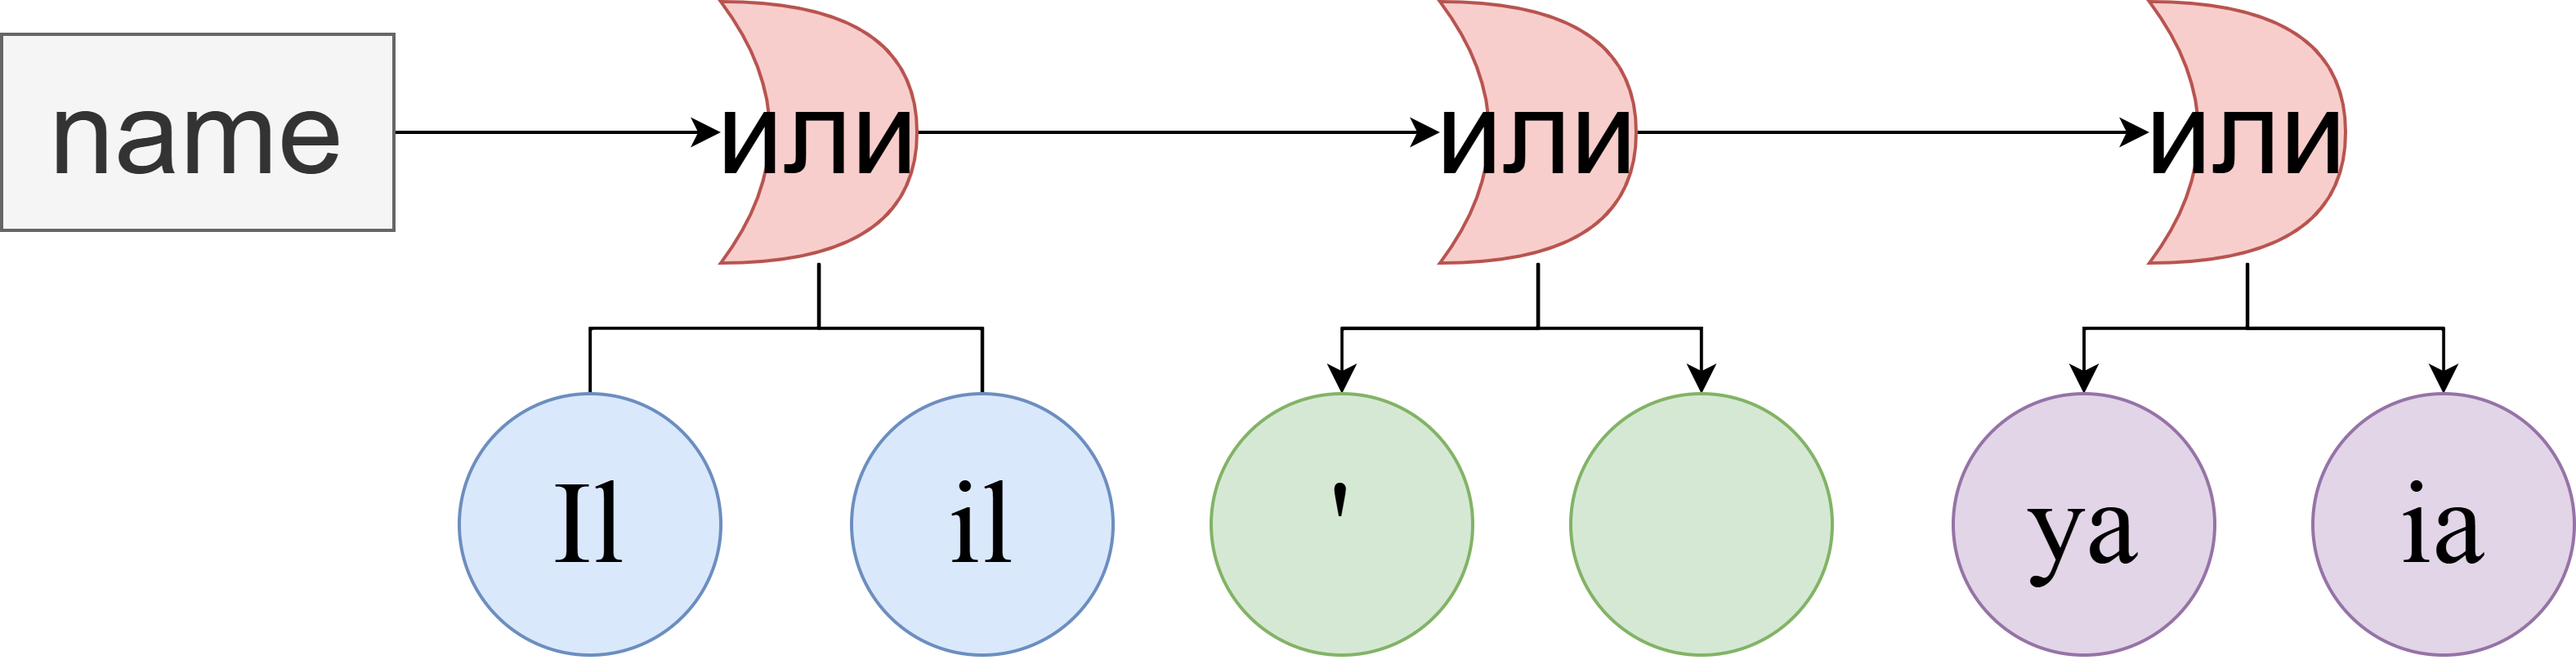
\includegraphics[width=0.45\textwidth]{graph-name}

\item Варианты написания фамилии - \path{db/graph/family.grd} размер - 85Б

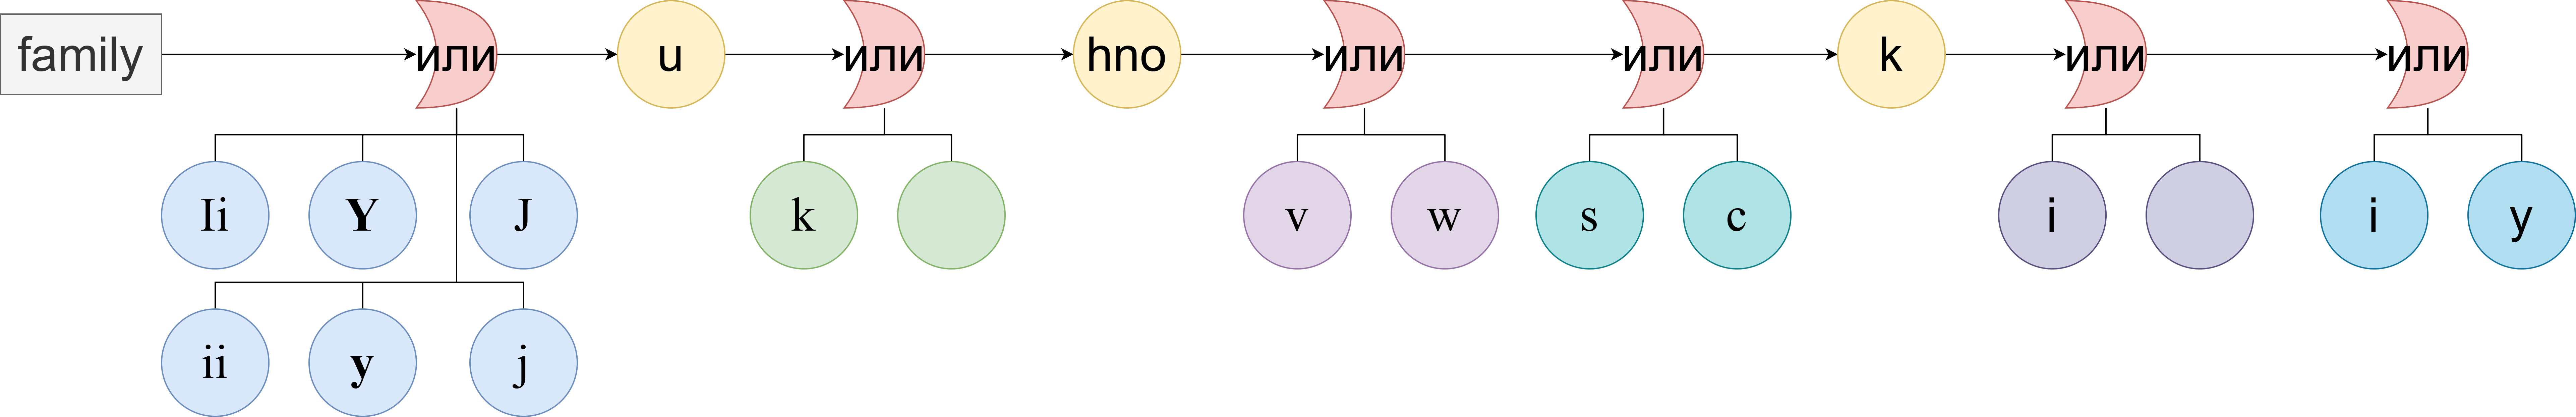
\includegraphics[width=1\textwidth]{graph-family}

\end{itemize}

Сожмем файлы и посмотрим на размер данных после сжатия:
\begin{lstlisting}
  ./src/utils/gzip/run.bat
\end{lstlisting}

Сожмем построчно текстовые файлы:
\begin{lstlisting}
  ./src/utils/gzip_rows/run.bat
\end{lstlisting}

Размеры файлов приведены в таблице \ref{files_size}

\begin{table}
\begin{center}
\begin{tabular}{|c|c|c|c|c|}
\hline
Представление \ Даные & name & family & $K_{name}$ & $K_{family}$\\
\hline
Текст (не сжатые) & 50 & 4670 & - & - \\
\hline
Текст (gzip файл) & 34 & 813 & 1,47 & 5,74 \\
\hline
Текст (gzip построчо) & 108 & 7192 & 0,46 & 0,65 \\
\hline
Граф (не сжатые) & 29 & 85 & 1,72 & 54,94 \\
\hline
Граф (gzip файл) & 32 & 84 & 1,56 & 55,59 \\
\hline
Граф (gzip построчно) & 73 & 196 & 0,69 & 23,83 \\
\hline
\end{tabular}
\end{center}
\caption{\label{files_size}Размер данных, где $K_{name}$, $K_{family}$} - коэффициеннты сжатия
\end{table} 

Из результатов видно, что сжатие на уровне блоков (построчно) не решает проблему избыточности между блоками и, следовательно, оставляет значительные возможности для улучшения сжатия, например с помощью графов. В нашем случае, графы построены по байтно, поэтому сжатие не дает никаких результатов. Графы дедуплицируют данные, поэтому мы получаем максимальнный коэффициент сжатия - 55,59.

Дедупликация стала популярной в системах резервного копирования для устранения дублирующегося контента во всем корпусе данных, часто достигая гораздо более высоких коэффициентов сжатия. Поток резервного копирования делится на фрагменты, и в качестве идентификатора каждого фрагмента используется устойчивый к коллизиям хэш (например, SHA-1). Система дедупликации поддерживает глобальный индекс всех хэшей и использует его для обнаружения дубликатов. Дедупликация хорошо работает как для основных, так и для резервных наборов данных, которые состоят из больших файлов, которые редко изменяются (а если и изменяются, то изменения редки).

К сожалению, традиционные схемы дедупликации на основе фрагментов не подходят
для операционных СУБД, где приложения выполняют запросы на обновление, которые изменяют отдельные записи. Количество дублирующихся данных в отдельной записи, скорее всего, незначительно. Но большие размеры фрагментов (например, 4–8 КБ) являются нормой, чтобы избежать огромных индексов в памяти и большого количества чтений с диска.

Рассмотрим дедупликацию на основе сходства \cite{Xu15} для
сжатия отдельных записей OLTP баз данных.

Вместо индексации каждого хеша фрагмента,
алгоритм выбирает небольшое подмножество хешей фрагментов для каждой новой записи базы данных, а затем использует этот образец для идентификации похожей записи в базе данных.

Затем он использует дельта-сжатие на уровне байтов для
двух записей, чтобы уменьшить как используемое онлайн-хранилище, так и пропускную способность удаленной репликации. dbDedup обеспечивает более высокие коэффициенты сжатия с меньшими накладными расходами памяти, чем дедупликация на основе фрагментов, и хорошо сочетается
со сжатием на уровне блоков, как показано на \ref{img1_xu17}. 

\begin{figure}[h]
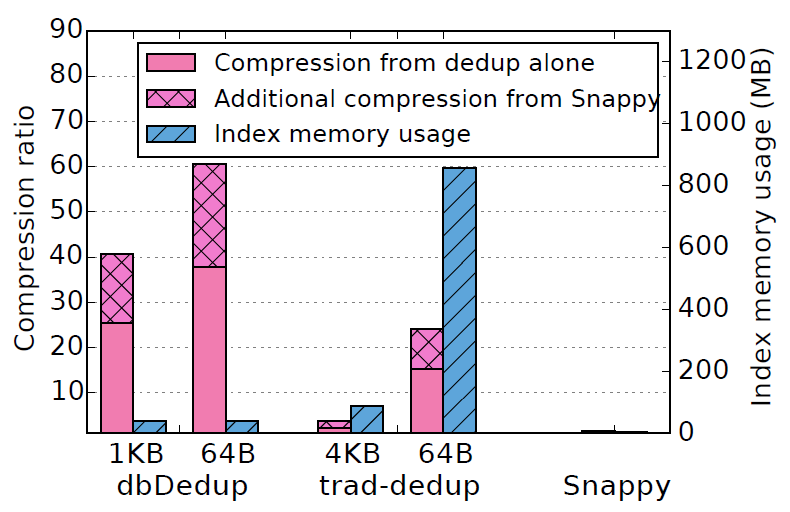
\includegraphics[width=0.75\textwidth]{img1_xu17}
\caption{\label{img1_xu17} Коэффициент сжатия и использование памяти индекса для данных Википедии,
хранящихся в пяти конфигурациях MongoDB: с dbDedup (размер фрагмента 1 КБ и 64 Б), с традиционной дедупликацией (4 КБ и 64 Б) и с Snappy (сжатие на уровне блоков). dbDedup обеспечивает более высокую степень сжатия и меньшие накладные расходы на память индекса, чем традиционная дедупликация. Snappy обеспечивает такое же сжатие 1,6 для данных после дедупликации или исходных данных. \cite{Xu17}}
\centering
\end{figure}

Авторы объединили несколько методов для достижения этой эффективности:
\begin{itemize}
    \item двустороннее кодирование для эффективной передачи закодированных новых записей (прямое кодирование) в удаленные реплики,
    \item сохраняя новые записи с закодированными формами выбранных исходных записей (обратное кодирование).
\end{itemize}

\section{ПРЕДЛОЖЕНИЕ}
Предлагается модифицировать алгоритм блочной дедупликации данных с последующим сжатием, описаный в \cite{Xu17}
\begin{figure}[h]
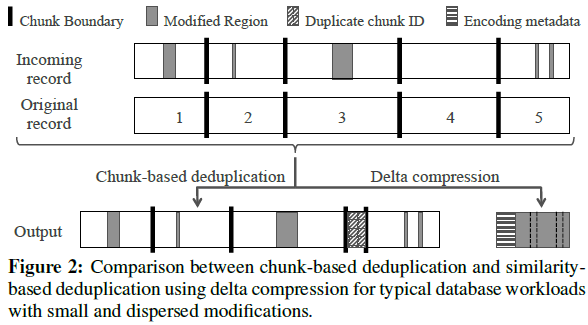
\includegraphics[width=0.75\textwidth]{alg_xu17}
\caption{\label{alg_xu17} Алгоритм блочной дедупликации, описаный в \cite{Xu17}}
\centering
\end{figure}

Но внести изменения - с помощью многомерной регресиии сворачивать различия похожих блоков в графы и храннить дельты в виде сжатых графовых векторов.

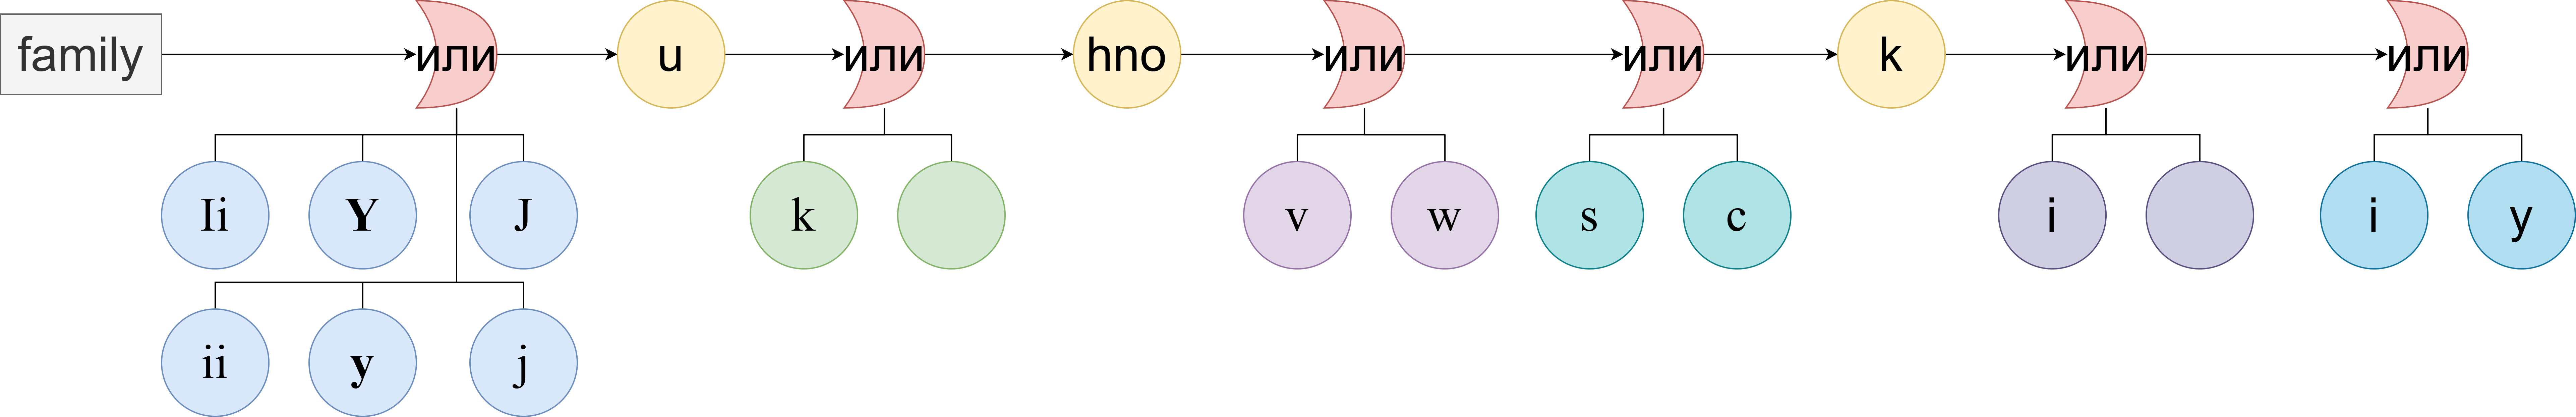
\includegraphics[width=1\textwidth]{graph-family}

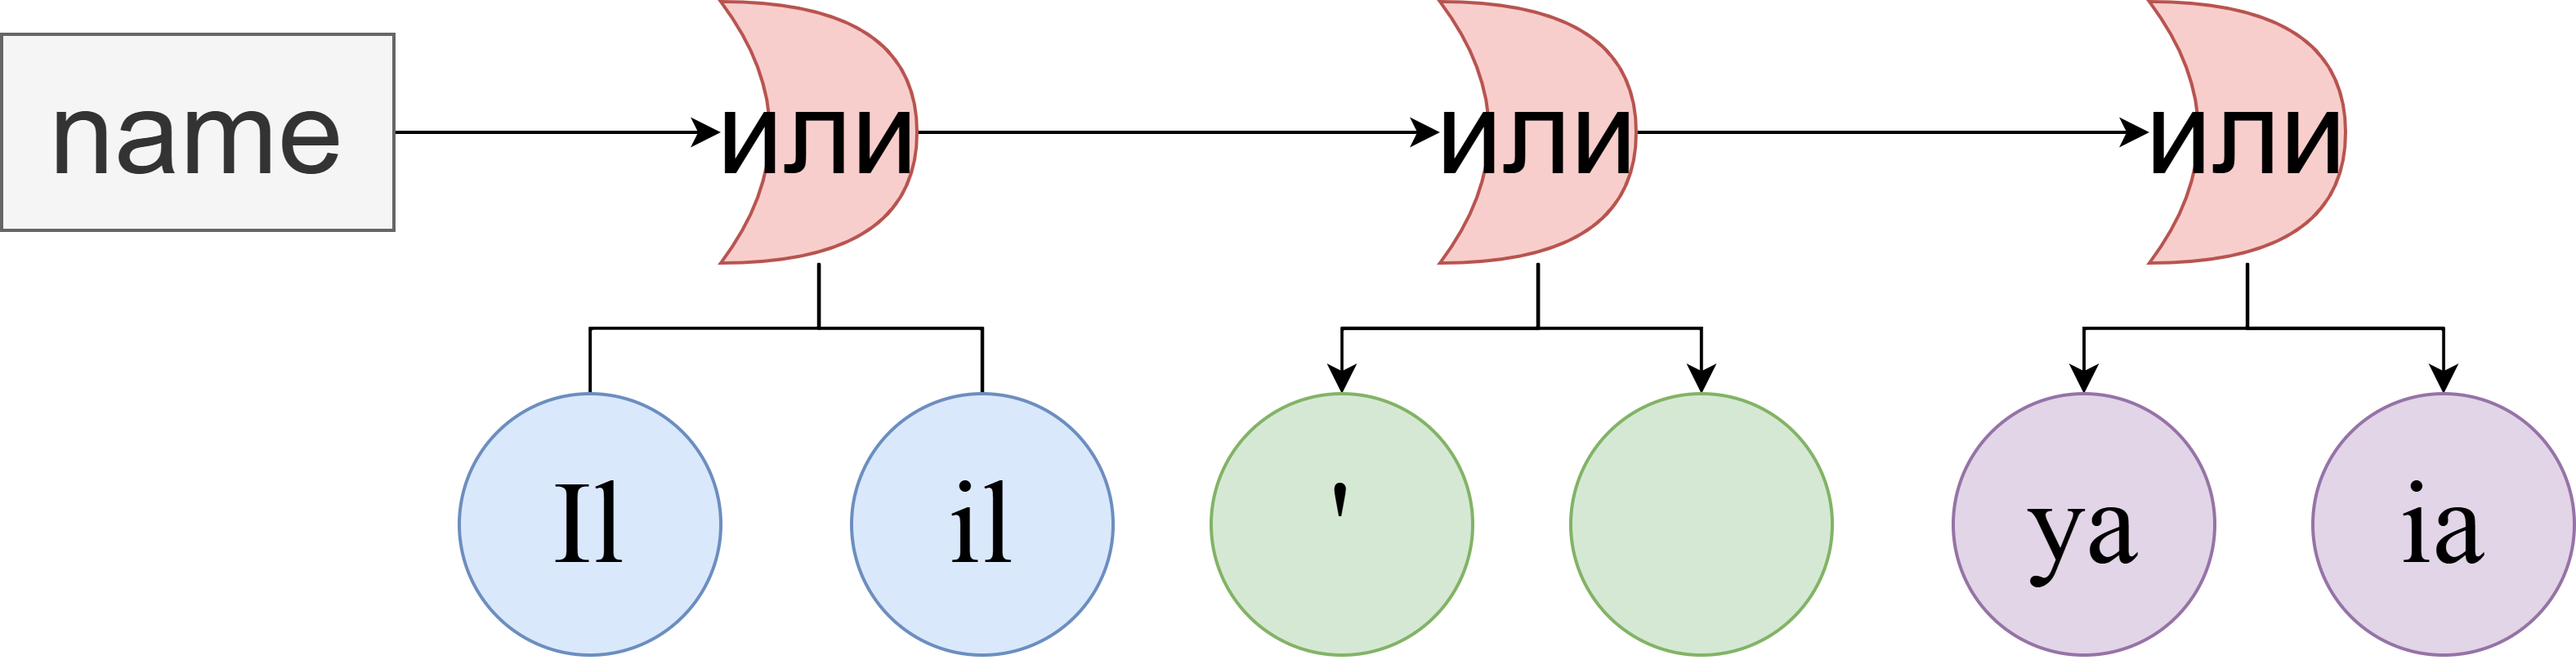
\includegraphics[width=0.45\textwidth]{graph-name}

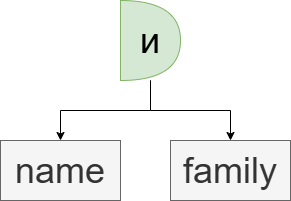
\includegraphics[width=0.15\textwidth]{graph-denormalized}

Данный подход позволит сжимать данные с коэффициеннтом более 50, что существенно сэкономит потребность в закупке нового оборудования.

\section{ЗАКЛЮЧЕНИЕ}
Использование ИИ в задачах, казавшихся достигших предела технических возможностей, приносит качественнные улучшения. Например, RoCE дало не только увеличение скорости передачи до 600GB, но еще и packetless network. Такой же эффект ожидается и от внедрения ИИ в алгоритмы дедупликации.

Для Заказчика это будет иметь коммерческий эффект в виде сокращения стоимости владениня хранилищ даных в десятки раз (до 60) и синжениня планов на закупки нового дорогостоящего оборудования - СХД, сетевая инфраструктура.

\section{ПРИЛОЖЕНИЕ}
\subsection{db/initial/name.dat - 50Б}
\verbatiminput{db/initial/name.dat}

\subsection{db/initial/family.dat - 7192Б}
\verbatiminput{db/initial/family.dat}

\subsection{db/graph/name.grd - 29Б}
\verbatiminput{db/graph/name.grd}

\subsection{db/graph/family.grd - 85Б}
\verbatiminput{db/graph/family.grd}

\subsection{src/utils/gzip/Compress.java}
\verbatiminput{src/utils/gzip/Compress.java}

\subsection{src/utils/gzip/run.bat}
\verbatiminput{src/utils/gzip/run.bat}

\subsection{CompressRows.java}
\verbatiminput{src/utils/gzip_rows/CompressRows.java}

\subsection{src/utils/gzip-rows/run.bat}
\verbatiminput{src/utils/gzip_rows/run.bat}

\begin{thebibliography}{9} 
    \bibitem{Cormack85} G. V. Cormack. Data compression on a database system. Communications of the ACM, 28(12):1336-1342, 1985.

    \bibitem{Iyer94} B. Iyer and D. Wilhite. Data compression support in databases. 1994.

    \bibitem{Xu15} L. Xu, A. Pavlo, S. Sengupa, J. Li, and G. R. Ganger.
Reducing replication bandwidth for distributed document
databases. In SoCC, pages 222–235, 2015.

  \bibitem{Xu17} Xu, L., Pavlo, A., Sengupta, S., and Ganger, G. R.(2017). Online Deduplication for Databases. In Proceedings of the 2017 ACM International Conference on Management of Data (SIGMOD 17) (pp.1355-1368). ACM Digital Library

\end{thebibliography}

\end{document}